\documentclass[11pt,a4paper]{article}
\usepackage[a4paper,margin=2cm]{geometry}
\usepackage[T1]{fontenc}
\usepackage[utf8]{inputenc}
\usepackage{lmodern}
\usepackage{microtype}
\usepackage{graphicx}
\usepackage{booktabs}
\usepackage{tabularx}
\usepackage{xcolor}
\usepackage[hidelinks]{hyperref}
\usepackage{caption}
\usepackage{enumitem}
\usepackage{titlesec}

\captionsetup{font=small,labelfont=bf,skip=4pt}
\setlist{nosep,leftmargin=1.2em}
\titleformat{\section}{\large\bfseries}{\thesection.}{0.5em}{}
\titleformat{\subsection}{\normalsize\bfseries}{\thesubsection}{0.5em}{}
\titlespacing*{\section}{0pt}{8pt}{3pt}
\titlespacing*{\subsection}{0pt}{6pt}{2pt}
\setlength{\parskip}{3pt}
\setlength{\parindent}{0pt}
\renewcommand{\arraystretch}{1.12}

\begin{document}

\begin{center}
{\LARGE\bfseries Research Paper Auditor}\\[3pt]
{\large An evidence-gated agent system for checking research papers}\\[6pt]
Final report, CL3.410 \quad|\quad Team Hood Research Department \quad|\quad 15 November 2026\\[4pt]
Vijay Aravynthan (2023111007) \quad Anurag Peddi (2023101090) \quad Itikela Bhaskar (2023111032) \quad Sudheera Y S (2023111002)\\[3pt]
Code: \url{https://github.com/itikelabhaskar/Research_Paper_auditor}
\end{center}

\section*{Abstract}
Reviewers rarely open the papers a submission cites or the code it releases, so a wrong
citation or a setting that differs from the code usually goes unnoticed. We built an auditor
that reads a paper (PDF or LaTeX) and its repository, splits it into checkable items, sends
each item to a specialist checker and reports a finding only with quoted evidence that a
verifier has found again in its source. We compared it with the same model in one pass
without tools (B0) and as one agent with all the tools (B1). On 40 paper--code pairs (80
paper versions, 163 planted errors, 72 clean controls) the full system reaches a Macro-F1 of
0.636 $\pm$ 0.004 over three runs, against 0.048 $\pm$ 0.015 for B0 and 0.046 $\pm$ 0.007 for
B1, and no system flags a clean control. It costs \$0.079 per paper version, against \$0.542
for B1. The weak points are clear too: it finds about a third of planted method changes, and
it raises 3.1 flags per unchanged paper that no label covers and that we have not yet judged
by hand. The citation checker scores F1 0.879 on the HALLMARK reference benchmark.

\section{Introduction}
Conferences now receive tens of thousands of submissions, and reviewers have no time to check
whether a cited paper really says what the citing sentence claims, or whether the reported
learning rate is the one in the released code. Language models make it easier to write a
plausible but wrong reference. Existing reference checkers only test that a reference exists;
prompted LLM reviewers read only the submission, so they cannot see what the cited paper or the
code says. Our proposal set one research question:

\textbf{RQ1.} Does an agent system that retrieves cited full texts and code repositories, and
tests each suspected error against them, detect more errors with fewer false alarms than the
same model run in a single pass? The target was at least 10 points more Macro-F1 than the
single-pass baseline, without more false alarms on clean papers.

Because a false accusation harms an author, every finding must carry a verbatim quote, and the
system must say when it cannot decide. Each output is one of three states: \emph{verified flag},
\emph{needs human review} or \emph{dropped}. A human makes every final decision.

The work was split into four parts: parsing, planning, orchestration and the baselines
(Bhaskar); the citation checker (Anurag); the code, data, template, theory and integrity
checkers (Vijay); and the verifier, report and evaluation (Sudheera). Table~\ref{tab:deliv}
lists what the proposal promised and what was delivered.

\begin{table}[h]
\centering\small
\caption{Proposal deliverables and their state.}
\label{tab:deliv}
\begin{tabularx}{\textwidth}{@{}lXl@{}}
\toprule
Promised & Delivered & State \\
\midrule
Planner, citation, code and template agents, verifier & All built, plus data, theory and integrity checkers; audit report and web UI & done \\
Baselines B0 and B1 & Both built on the same model, tools and budgets & done \\
Set A (HALLMARK) & 831 references scored & done \\
Set B, about 600 claim--source pairs & 60 papers, 159 labels; full-system run on all of it not done & partial \\
Set C, 160 paper--code instances & 40 pairs, 80 versions, 235 labels; all systems run & done (smaller) \\
Metrics: Macro-F1, false alarms, grounding, cost & All four reported by one scorer (\texttt{auditor evaluate}) & done \\
Ablation: remove the verifier & Scored on every full-system run & done \\
Ablation: abstract-only retrieval & Only on B1 subsets; full-system run needs credits & partial \\
Recall@5 of the gold passage & Measured on the 6 set B records that have one & partial \\
Tool-call accuracy & Not measured & not done \\
Three runs of each system & Full system and B0 three, B1 two (spend limit) & partial \\
\bottomrule
\end{tabularx}
\end{table}

\section{Literature review}
\textbf{Reference checking.} HALLMARK~\cite{hallmark} is a benchmark of fabricated and corrupted
BibTeX entries (wrong venue, near-miss titles, merged citations and so on). It tests whether a
verifier can tell a real reference from a bad one, and by design not whether the cited work
supports the sentence citing it. We use its public test split as our set A.

\textbf{Claim verification.} SciFact~\cite{scifact} frames checking a scientific claim against an
abstract as retrieval plus entailment. We follow the same idea but go further: we retrieve the
cited paper's full text where it is open, rank its passages with BM25~\cite{bm25}, and require
the model to quote the passage it relies on. Retrieval-augmented generation~\cite{rag} and
tool-using agents such as ReAct~\cite{react} are the general patterns behind our specialists and
behind baseline B1.

\textbf{LLM reviewers.} Liang et al.~\cite{liang} found that GPT-4 feedback on papers overlaps
with human reviews, but such reviewers see only the submission. Google's Paper Assistant
Tool~\cite{pat} is an agent that reads a whole manuscript and checks its theory and experiments;
on SPOT's mathematics subset it reports 89.7\% of errors found, against 55.2\% for a single
Gemini 3.1 Pro call. SPOT~\cite{spot} collects real errors that led to errata or retractions; we
use its mathematics and computer science papers as our theory test.

\textbf{Paper--code consistency.} SciReplicate-Bench~\cite{scireplicate} asks models to write code
from a paper's method, which is a different task. SciCoQA~\cite{scicoqa} pairs papers with their
official code and lists real and synthetic discrepancies between them. Our set C is built from
SciCoQA pairs. For statistics inside a paper we use the GRIM test~\cite{grim}, which shows when a
mean of integer data is impossible for the stated sample size.

None of these systems checks references, claim support, code and the paper's own numbers
together, and none refuses to report a finding it cannot back with a quote. That combination is
what we tested.

\section{Datasets}
We used two public benchmarks and built three sets of our own (Table~\ref{tab:data}). A
\emph{pair} is a paper with its official code. Our sets keep each paper twice: the original and a
copy with planted errors. \emph{Clean controls} are labelled items we left unchanged, so a flag on
one is a false alarm. Planted errors were made by scripts that propose an edit and then check it
(for example, a changed number must not appear in the cited source, and a fabricated title must
resolve to nothing), so a label is only kept if the error can really be found. A second person
reviewed 20\% of the labels of sets B and C (decision D18).

\begin{table}[h]
\centering\small
\caption{Evaluation sets. Counts are from the committed label files.}
\label{tab:data}
\begin{tabularx}{\textwidth}{@{}>{\raggedright\arraybackslash}p{2.7cm}>{\raggedright\arraybackslash}p{3.6cm}>{\raggedright\arraybackslash}X>{\raggedright\arraybackslash}p{3.1cm}@{}}
\toprule
Set & What it tests & Size & Labels from \\
\midrule
A: HALLMARK~\cite{hallmark} & Reference exists, metadata right & 831 entries (524 corrupted, 307 valid) & released \\
B: claim--source & Citations: existence, metadata, support, numbers & 60 arXiv papers (cs.LG, cs.CL, 2025); 113 planted (96 not found, 9 metadata, 5 unsupported, 3 number), 46 clean & injection log; 34 reviewed \\
C: paper--code (SciCoQA) & Settings, metrics and method against the code & 40 pairs, 80 versions; 60 setting, 3 metric, 100 method, 72 clean & injection log, SciCoQA; 47 reviewed (all agreed) \\
D: integrity plants & Placeholder text, impossible means, text against tables, broken code & the 40 set C papers; 195 plants & templates; not reviewed \\
SPOT~\cite{spot} & Errors in proofs and derivations & 26 papers, 29 errors; dev and test halves of 13 & released, LLM judges \\
Parser fixtures & Citation linking & 10 arXiv papers, 797 markers, 100 checked by hand & hand \\
\bottomrule
\end{tabularx}
\end{table}

Set B came out smaller than the 600 pairs we planned: after the propose-and-verify step and three
rounds of corrections, 159 labels remained, and only 8 test claim support or numbers. Set C has
92 method discrepancies (8 reported by users, 84 synthetic); the 8 reported ones exist in both
copies of a paper, which gives 100 method labels. No set C item tests the data classes (splits,
sizes, labels, leakage), so the data checker is only tested on fixtures.

\section{Methodology}
\begin{figure}[t]
\centering
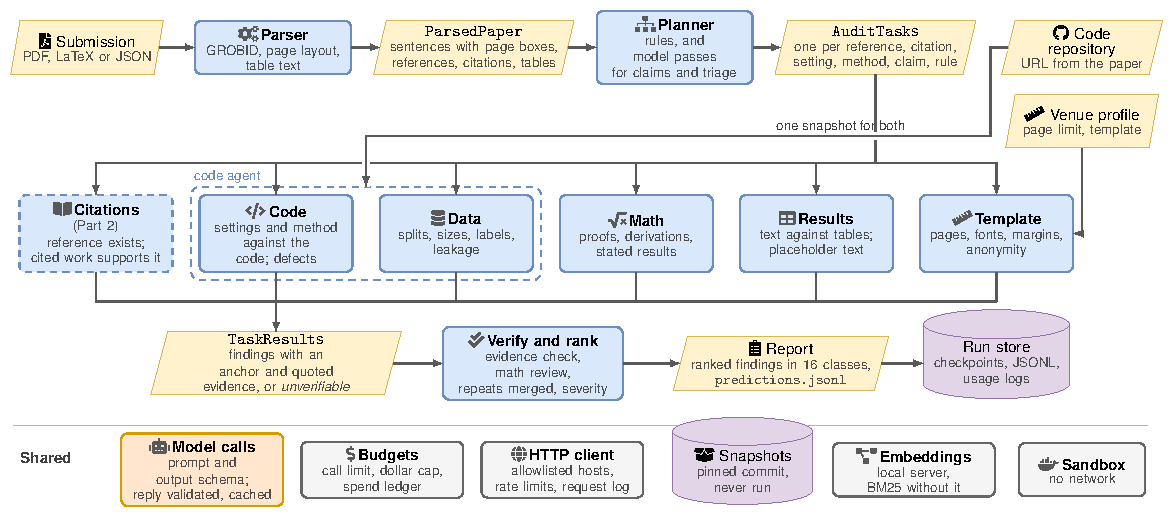
\includegraphics[width=\textwidth]{../docs/figures/system.pdf}
\caption{The auditor. The parser turns the submission into sentences with page boxes; the planner
makes one task per reference, citation, stated setting, method, claim and venue rule; each task
goes to the checker for its kind. Every finding names its sentence or code lines and quotes its
evidence, and the verifier checks that evidence before anything is reported.}
\label{fig:system}
\end{figure}

Figure~\ref{fig:system} shows the pipeline. All records passed between stages are frozen Pydantic
models, so a malformed finding fails at once instead of reaching the report.

\textbf{Parsing.} PDFs go through GROBID~\cite{grobid}, which gives sentences, references and
citation markers; LaTeX sources are parsed directly. GROBID's tables lose numbers, so we also read
the PDF text inside each table's region, which recovers 96\% of table numbers on 39 papers
against 57\% for GROBID alone. A fallback linker resolves author--year markers GROBID leaves
open: 765 of 797 markers (96\%) on our 10 fixture papers are linked, and 99 of 100 checked by hand
are linked correctly.

\textbf{Planning.} Rules turn the paper into tasks: one per reference, per citing sentence, per
stated setting (batch size, learning rate, epochs and so on), per method section, per numeric
claim and per venue rule. An optional model pass narrows each citation's claim. A set C paper
gives about 166 tasks.

\textbf{Specialists.} Each checker returns either findings with evidence or an \emph{unverifiable}
result with a reason; it never guesses.
\begin{itemize}
\item \emph{Citations.} References are looked up by DOI, arXiv id or title in Crossref, OpenAlex,
arXiv and Semantic Scholar, and their title, authors, year and venue are compared. For a citing
sentence, the cited work's full text (arXiv HTML or the PDF through GROBID, else the abstract) is
split into passages, the top five are ranked by BM25, and the model judges support and quotes
one passage. A number the claim gives is compared with the source's number in code, not by the
model.
\item \emph{Code and data.} Static scanners read every value of a setting from the repository
snapshot (pinned to a commit, never executed); a model is asked only when the comparison cannot
decide which value belongs to the paper's experiment. For the method, each sentence retrieves the
most similar code chunks with nomic embeddings~\cite{nomic} and the model compares them. A
finding is kept only if its code lines were really shown to the model.
\item \emph{Theory.} Two triage calls pick up to four claims per paper, a deep check reads each
claim with the whole paper (and may test it in a sandbox with no network), and a last call drops
findings that are refuted.
\item \emph{Integrity and template.} Rules with no model: leftover placeholder text, GRIM, text
that contradicts its own table, and venue rules (pages, fonts, margins, anonymity).
\end{itemize}

\textbf{Verifier.} Every quote must be found again in its source: the paper's sentence, the cited
work's text or the code lines. A finding whose evidence is missing goes to human review; one whose
evidence is refuted is dropped. Findings that rest on something \emph{not} being found (a
reference that resolves to nothing) always go to human review. Repeats are merged and each flag
gets a severity. An optional second model reading of support and method findings exists but was
off in our runs.

\textbf{Orchestration and cost control.} A LangGraph~\cite{langgraph} graph runs the checkers in parallel with
retries, checkpoints (a stopped run resumes), a call budget per task, a dollar cap per run and a
shared spend ledger across runs. Scholarly API and model replies are cached.

\textbf{Baselines.} B0 is the same model reading the whole paper once, with no tools. B1 is one
agent with every tool the specialists use, up to 20 model calls, and no verifier. Both use the
same error classes and answer format.

\textbf{Scoring.} A prediction matches a label when it names the same paper, anchor (sentence,
reference or code location) and target. Each label matches at most one prediction. For the full
system only verified flags count; for B0 and B1 every flag counts. Macro-F1 averages F1 over the
error classes present in the labels. A flag on a clean control is a false positive. A flag that
matches no label is counted separately as \emph{unlabelled}, because it may be a real error we did
not plant; we also report flags per unchanged original paper. \emph{Grounding} is the share of
flags whose quotes are found verbatim in their sources.

\section{Experiment runs}
All main runs used Gemini 3.8 Flash on Vertex AI for every system, the method check in retrieval
mode, and the same code version (hash \texttt{88b2408fee}). The citation checker was switched off
on set C because set C has no citation labels; it was recorded as a placeholder for both the full
system and B1, so the two stay matched. The full system and B0 ran three times and B1 twice; a
third B1 run stopped at the shared \$125 spend limit after 10 of 80 versions and is not scored.
Every paper version finished in every scored run.

\begin{table}[h]
\centering\small
\caption{RQ1 on set C (80 versions, 163 planted errors, 72 clean controls). Mean $\pm$ sample
standard deviation over runs. Source: \texttt{results/p4/set\_c-rq1.md}.}
\label{tab:rq1}
\begin{tabular}{@{}lcccc@{}}
\toprule
 & Full system & No verifier & B0 & B1 \\
\midrule
Runs & 3 & 3 & 3 & 2 \\
\textbf{Macro-F1} & \textbf{0.636 $\pm$ 0.004} & 0.667 $\pm$ 0.003 & 0.048 $\pm$ 0.015 & 0.046 $\pm$ 0.007 \\
Recall & 0.368 & 0.415 & 0.029 & 0.028 \\
Precision on labelled items & 1.000 & 1.000 & 1.000 & 1.000 \\
F1: method / metric / setting & 0.34 / 0.80 / 0.77 & 0.34 / 0.80 / 0.86 & 0 / 0 / 0.14 & 0 / 0 / 0.14 \\
Clean controls flagged & 0 of 72 & 0 of 72 & 0 of 72 & 0 of 72 \\
Flags per unchanged original & 3.12 & 4.71 & 1.63 & 0.39 \\
Unchanged originals with a flag & 94\% & 95\% & 76\% & 21\% \\
Unlabelled flags per run & 255 & 391 & 125 & 29 \\
Flags backed by evidence & 100\% & 100\% & 0\% & 0\% \\
Model calls per version & 13.2 & 13.2 & 1.0 & 20.1 \\
Cost per version & \$0.079 & \$0.079 & \$0.047 & \$0.542 \\
\bottomrule
\end{tabular}
\end{table}

The full system beats B1 by 59.0 points and B0 by 58.8 points of Macro-F1, so the +10 point target
is met by a wide margin. Neither baseline finds a single method or metric error, and each finds
only 3 to 6 of the 60 changed settings. The full system is also cheaper than B1: B1 sends the
whole paper with each of its 20 calls, about 670,000 input tokens per paper version. All set C
runs together cost \$125.04 (full system \$18.84 for three runs, B0 \$11.35, B1 \$86.78 for two,
plus a \$1.70 pilot and \$6.36 for the stopped B1 run), priced at list rates.

The second half of the target, no more false alarms on clean papers, is not settled. No system
flags a clean control item, but on the unchanged originals the full system raises 3.1 flags per
paper against 1.6 for B0 and 0.4 for B1. Some are real discrepancies already in these papers
(SciCoQA includes user-reported ones); the rest are false alarms. In each run 68 to 71 of the 124
to 127 verified flags on originals were ``unfinished text'', almost all sentences that GROBID cut
at an abbreviation such as ``Fig.''. Such findings now go to human review (10 November), so these
runs overstate what the current code flags.

\textbf{Where planted errors are lost.} Over the three full runs (489 planted-error instances),
180 were verified, 26 went to human review because the checker marked them uncertain, 48 ended
unverifiable and 235 got no matching finding. Almost all of the last group are method changes: in
a separate check of 57 method misses, 26 were in code the model was shown but did not report, 14
were never retrieved and 7 were removed by the evidence gate. Lost settings are the conservative
kind: 45 times every repository value of the setting was judged to belong to a different
experiment, so the task ended unverifiable instead of raising a wrong flag. Of the 163 planted
errors, the full system finds 57 in all three runs and 99 in none.

\section{Ablations}
\textbf{Removing the verifier} (proposal ablation for reasoning). Every candidate finding of the
three full runs was also scored without the verifier (Table~\ref{tab:rq1}). Taking it out raises
Macro-F1 from 0.636 to 0.667 but unlabelled flags from 255 to 391 per run, and flags per original
paper from 3.1 to 4.7. Over the three runs the verifier verified 180 of the 203 findings that match
a planted error, sent 23 to review and dropped none; it dropped nothing at all, because every quote
the specialists gave was found again in its source. So on set C it trades 3.1 points of F1 for 35\%
fewer unlabelled flags. Whether that is a gain in precision depends on how many of the held-back
flags are false alarms, which needs the hand check we have not done. Counting the uncertain findings
as flags would give 0.668, 0.668 and 0.663.

\textbf{Model only, and one agent with tools} (proposal ablations for tool calling and agentic
abilities). These are baselines B0 and B1 in Table~\ref{tab:rq1}. Tools alone (B1) did not help: B1
scores no better than B0 at eleven times the cost.

\begin{table}[h]
\centering\small
\caption{Smaller ablations, each changing one component.}
\label{tab:abl}
\begin{tabularx}{\textwidth}{@{}>{\raggedright\arraybackslash}X>{\raggedright\arraybackslash}X>{\raggedright\arraybackslash}p{4.2cm}@{}}
\toprule
Question & Variants & Result \\
\midrule
Finding the code for a method sentence (84 known differences; changed line shown) & word overlap / BM25 / nomic embeddings / BM25+embeddings / +reranker & 35 / 48 / \textbf{59} / 57 / 57 \\
Model reading the code (57 known differences found) & 3.8 Flash / 3.1 Pro / DeepSeek V4.1 / Kimi K2 / GLM-5 / 3.5 Flash-Lite & 17 / 19 / 19 / 13 / 11 / 7 \\
Code shown to the model (57 differences) & 60k / 120k characters & 17 / 16 \\
Reading tables from a PDF (numbers recovered, 12 papers) & GROBID / layout text / both / text in table region / page image & 41 / 20 / 51 / \textbf{98} / 96\% \\
Citation passage ranking (Recall@5, 6 records) & BM25 / MiniLM embeddings & \textbf{6} / 4 of 6 \\
Citation fixes on set A (author, year, venue rules) & before / after & FPR 31\% / 16\%; F1 0.80 / 0.88 \\
Claim-loop effort (3 papers) & medium / low with a time limit per claim & 17--32 / \textbf{0} timeouts; \$0.63 / \$0.47 \\
Theory checker shape (SPOT test half, first judge) & triage then deep check / two triage calls pooled & \textbf{8} / 7 of 14 \\
\bottomrule
\end{tabularx}
\end{table}

\textbf{Abstract-only retrieval} (proposal ablation for RAG). We only ran it with B1 on a subset of
set B, where full text and abstract both gave Macro-F1 0.026; B1 found almost nothing either way, so
this says nothing about the full system. The full-system run on set B was not done (Section 8).

Two other results from Table~\ref{tab:abl} shaped the final system: embedding search was kept for
method retrieval, and BM25 was kept for citation passages because it matched or beat MiniLM on the
few gold passages we have (6 of 6 against 4 of 6; the gold passages were picked from BM25's top
result, which favours it). A stronger reading model helped little: the best two find 2 more of 57
than Gemini 3.8 Flash at three to four times the cost.

\section{Evaluations of the individual checkers}
\begin{table}[h]
\centering\small
\caption{Checker-level results.}
\label{tab:checkers}
\begin{tabularx}{\textwidth}{@{}>{\raggedright\arraybackslash}X>{\raggedright\arraybackslash}p{5.4cm}>{\raggedright\arraybackslash}p{4.4cm}@{}}
\toprule
What we test & Result & Notes \\
\midrule
Set A: reference corrupted or fake (831 entries) & F1 0.879, P 0.902, R 0.857 & 49 of 307 valid flagged (16\%) \\
Citation marker linked to a reference (10 papers) & 96\% (765 of 797) & 99 of 100 correct by hand \\
Set C settings, static check only & 100\% (60 of 60) & 0 of 72 clean controls flagged \\
Set C metrics, static check only & 67\% (2 of 3) & \\
Set D placeholder text / GRIM-impossible mean & 100\% (40 of 40) / 100\% (40 of 40) & \\
Set D reversed comparison / wrong gain & 94\% (31 of 33) / 55\% (18 of 33) & \\
Set D number differs from its table & 20\% (2 of 10) & no false alarm on 254 real papers \\
Set D undefined name / syntax error in code & 100\% (26 of 26) / 100\% (13 of 13) & \\
Template rules (hand-built fixtures) & 100\% (15 of 15) & \\
SPOT proof errors, test half & 57\% (8 of 14) one judge; 36\% (5 of 14) both & \$1.68 for 13 papers \\
\bottomrule
\end{tabularx}
\end{table}

The rule-based checks are strong on what they were built for, but set D plants come from our own
templates, so these numbers are an upper bound for real papers. The weakest HALLMARK types are
nonexistent venues (recall 0.38) and preprints cited as published (0.50). On SPOT, the two LLM judges
disagree on several matches, so we report both counts; Google's tool reports 55.2\% for one call on
the same subset~\cite{pat}, with a stronger model. On real papers the checks found, for example, a
reversed comparison in arXiv 2312.11580 (``PlaNet-S (0.73) is higher than U-Net (0.78)'') and a code
loader that shuffles in arXiv 2006.06958, whose text says no shuffling is used.

\section{Limitations}
\begin{itemize}
\item \textbf{False alarms on clean papers are not judged.} The full system flags 94\% of unchanged
originals. We planned to check a sample by hand (task S5) and did not finish it, so we cannot claim
the ``no more false alarms'' half of RQ1.
\item \textbf{Set B was not run end to end.} We ran out of model credits. Also, the verifier sends every
``reference not found'' finding to human review, and 96 of set B's 113 planted errors are of that
class, so under our own scoring rule the full system could score at most the other 17.
\item \textbf{Small classes.} Set C has only 3 metric errors and set B only 8 claim labels, so their
F1 can move a lot with one item. The data classes are not tested on a labelled set.
\item \textbf{Labels.} All planted errors are synthetic except the 8 reported SciCoQA discrepancies. The
set B second review was done by an agent session that Anurag set up as reviewer, not by a teammate;
set D has no second review; SPOT matches are graded by LLM judges with no human check.
\item \textbf{One model family.} All main runs use Gemini 3.8 Flash; B1 has two runs, not three.
\item \textbf{Method recall is low.} The method F1 is 0.34, and most misses are code the model saw but
did not report.
\item \textbf{Parsing.} GROBID splits sentences at abbreviations; we did not change it because the gold
labels point at sentence ids.
\item \textbf{Cost.} Costs are priced at Gemini list rates; our bill matched full price for cached input.
\end{itemize}

\section{Conclusions}
On paper--code consistency, checking each item with tools and a quote-based verifier works far
better than the same model reading the paper or acting as one tool-using agent: Macro-F1 0.636
against under 0.05, at a seventh of B1's cost, with no clean control flagged and every flag backed by
evidence found in its source. The verifier removes about a third of the unlabelled flags for 3 points
of F1. What we cannot yet say is how many of the 3 flags per clean paper are real problems, and the
citation side has only been tested on its own and on the HALLMARK benchmark, not end to end on set
B. Both are the next steps, together with better recall for method changes.

\textbf{Reproducibility.} The repository README lists setup (\texttt{uv sync}, GROBID in Docker), the
commands to audit a paper, run a batch and score it (\texttt{auditor audit}, \texttt{auditor batch},
\texttt{auditor evaluate}), and a web UI. The set C experiment settings are in
\texttt{configs/experiments/set\_c.env}, the runs in \texttt{results/p4/runs}, and
\texttt{auditor evaluate} re-scores them without any model call. Over 1,380 offline tests run on
Windows, Linux and macOS.

\begin{thebibliography}{99}\small
\bibitem{hallmark} HALLMARK: Diagnosing three failure modes in LLM citation verifiers. arXiv:2607.18360, 2026. Data: \url{https://github.com/rpatrik96/hallmark}.
\bibitem{spot} G.~Son et al. When AI co-scientists fail: SPOT, a benchmark for automated verification of scientific research. arXiv:2505.11855, 2025.
\bibitem{scicoqa} T.~Baumg\"artner and I.~Gurevych. SciCoQA: Quality assurance for scientific paper--code alignment. arXiv:2601.12910, 2026.
\bibitem{pat} R.~Jayaram et al. Towards automating scientific review with Google's Paper Assistant Tool. arXiv:2606.28277, 2026.
\bibitem{scireplicate} Y.~Xiang, H.~Yan, S.~Ouyang, L.~Gui and Y.~He. SciReplicate-Bench: Benchmarking LLMs in agent-driven algorithmic reproduction from research papers. COLM 2025. arXiv:2504.00255.
\bibitem{scifact} D.~Wadden, S.~Lin, K.~Lo, L.~L.~Wang, M.~van Zuylen, A.~Cohan and H.~Hajishirzi. Fact or fiction: Verifying scientific claims. EMNLP 2020, pp.~7534--7550.
\bibitem{liang} W.~Liang et al. Can large language models provide useful feedback on research papers? A large-scale empirical analysis. NEJM AI 1(8), 2024.
\bibitem{rag} P.~Lewis et al. Retrieval-augmented generation for knowledge-intensive NLP tasks. NeurIPS 2020.
\bibitem{react} S.~Yao et al. ReAct: Synergizing reasoning and acting in language models. ICLR 2023.
\bibitem{bm25} S.~Robertson and H.~Zaragoza. The probabilistic relevance framework: BM25 and beyond. Foundations and Trends in Information Retrieval 3(4):333--389, 2009.
\bibitem{grobid} P.~Lopez. GROBID: Combining automatic bibliographic data recognition and term extraction for scholarship publications. ECDL 2009, LNCS 5714, pp.~473--474.
\bibitem{nomic} Z.~Nussbaum, J.~X.~Morris, B.~Duderstadt and A.~Mulyar. Nomic Embed: Training a reproducible long context text embedder. Transactions on Machine Learning Research, 2025. arXiv:2402.01613.
\bibitem{grim} N.~J.~L.~Brown and J.~A.~J.~Heathers. The GRIM test: A simple technique detects numerous anomalies in the reporting of results in psychology. Social Psychological and Personality Science 8(4):363--369, 2017.
\bibitem{langgraph} LangChain. LangGraph. \url{https://github.com/langchain-ai/langgraph}.
\end{thebibliography}

\appendix
\section{Team contributions}
\begin{tabularx}{\textwidth}{@{}lX@{}}
\toprule
Member & Work \\
\midrule
Itikela Bhaskar & Parser (GROBID, LaTeX, table regions, citation linking), planner, LangGraph orchestration with budgets, checkpoints and the spend ledger, baselines B0 and B1, batch runner, shared schemas, Docker image, failure analysis of Part 1 \\
Anurag Peddi & Citation checker (lookup in four indexes, full-text retrieval, passage ranking, support and number checks), set A scoring, set B construction and review \\
Vijay Aravynthan & Code, data, template, theory and integrity checkers, the claim loop, sets C and D, SPOT scoring and most ablations \\
Sudheera Y S & Verifier, audit report, the evaluation runner (\texttt{auditor evaluate}), the set C experiments and their analysis \\
\bottomrule
\end{tabularx}

\section{Per-run results on set C}
{\small\setlength{\tabcolsep}{3pt}
\begin{tabular}{@{}llrrrrr@{}}
\toprule
Run & System & Macro-F1 & Found & Missed & Unlabelled & Cost \\
\midrule
r1 / r2 / r3 & full & 0.641 / 0.636 / 0.632 & 61 / 60 / 59 & 102 / 103 / 104 & 251 / 245 / 268 & \$6.26 / 6.30 / 6.28 \\
r1 / r2 / r3 & B0 & 0.051 / 0.061 / 0.032 & 5 / 6 / 3 & 158 / 157 / 160 & 104 / 140 / 132 & \$3.68 / 3.74 / 3.93 \\
r1 / r2 & B1 & 0.042 / 0.051 & 4 / 5 & 159 / 158 & 43 / 14 & \$42.59 / 44.19 \\
\bottomrule
\end{tabular}}

\end{document}
